\chapter{Results}
\label{ch:results}
\textit{This chapter presents the results of the project, based on both qualitative and quantitative data. The goal is to provide insight into how the monitoring dashboard performs in terms of usability, functionality, and user experience.}

\textit{We begin by reviewing the qualitative results from our prototype and \acrshort{mvp} user tests. These results are based on hands-on sessions where participants interacted with the system and shared their feedback during and after completing realistic usage scenarios. Their input helped us identify usability issues and informed the final design.}

\textit{Next, we present the quantitative findings based on the \acrfull{sus}. This gives us a measurable indication of how users perceived the system’s ease of use. While \acrshort{sus} scores are not statistically precise with small samples, they still offer valuable insight, especially when paired with the qualitative feedback from our user tests.}

\textit{Together, these results allow us to assess how well the system supports its intended users, and whether it meets the practical and technical goals defined earlier in the project.}

\section{Results from Qualitative Data}
\textit{The first part of the results presents feedback from our user tests of both the prototype and the minimum viable product (\acrshort{mvp}). Each session was based on a predefined task script, and the participants shared their thoughts during and after completing the tasks. Their responses highlighted both strengths and areas for improvement, and these observations shaped our final design decisions.}

\subsection{Requirement‑elicitation results}
\label{subsec:req_results}

We went through four rounds of requirement gathering throughout the project. Each round added new insight and helped shape the system to better fit real user needs. The full requirement lists are included in \hyperref[sec:req_gathering]{Requirement Elicitation}, but Table~\ref{tab:req_evolution_table} below highlights the main changes introduced in each step.

\section*{Functional requirements}
\begin{table}[H]
    \centering
    \renewcommand{\arraystretch}{1.3}
    \resizebox{\textwidth}{!}{
    \begin{tabular}{|>{\RaggedRight\arraybackslash}p{4.5cm}|>{\RaggedRight\arraybackslash}p{10.5cm}|}
        \hline
        \textbf{Development Phase} & \textbf{Main Outcome} \\
        \hline
        \textbf{Assignment brief} (\ref{app:req-headspin-brief}) & Defined the initial scope with six functional (F1–F6) and four non-functional (NF1–NF4) requirements. \\
        \hline
        \textbf{Stakeholder meeting} (\ref{app:stakeholder}) & Clarified user roles and introduced personal dashboards, resulting in two new functional requirements (F7–F8). \\
        \hline
        \textbf{Prototype test} (\ref{app:req-prototype}) & Identified the need to adjust UI colours, add filter and sort functionality (F9), and improve text readability (NF5). \\
        \hline
        \textbf{MVP user test} (\ref{app:req_mvp_user_test}) & Added support for configurable alert thresholds (F10) and introduced a performance constraint (NF6). \\
        \hline
    \end{tabular}
    }
    \caption{Key changes in system requirements across development phases}
    \label{tab:req_evolution_table}
\end{table}

Each round of development helped us to understand more clearly what the dashboard needed to do and who it was really for. The assignment brief gave us a technical foundation to build on, the stakeholder meeting helped clarify actual user roles and expectations, and the prototype test highlighted some of the first user interface challenges. The \acrshort{mvp} test added another layer, showing what kind of performance was expected and which alert settings users needed more control over. Together, these steps helped shape the final set of requirements included later in the chapter.

\subsection{User Test of Prototype}
Each prototype test was based on a predefined scenario designed to explore early design ideas and core functionality. During the session, the scenario was read aloud while participants interacted with the prototype. A full description of the test setup is provided in the methodology section (Section ?), and the script is included in Appendix [XX].

\subsubsection{\textit{\textbf{User test: participant 1}}}
The first participant commented that everything appeared too green and lacked visual distinction. Filtering and sorting controls were expected at the top of the screen, and more actions should be available directly from the dashboard. The participant asked for more compact ways to show relevant data, ideally through visual elements instead of expanding the layout. Metrics like response time in milliseconds and uptime percentages over different time ranges (day, month, year) were seen as important for getting a quick overview. Given the limited number of navigation options, the sidebar was seen as unnecessary, and a top-mounted menu was preferred. The participant wanted each card to display multiple data dimensions at once, increasing its immediate information value without extra clicks.

\subsubsection{\textit{\textbf{User test: participant 2}}}
The second participant described the interface as “very green” and somewhat cluttered. A list view was preferred over the current card layout, and visual elements such as graphs were expected to help present site status more clearly. Historical uptime data (weekly, monthly, or yearly) per site was considered essential for understanding trends. In each card, the participant expected to find the responsible adviser, developer, customer information, and the site’s favicon. Without these elements, the layout felt incomplete and made it harder to identify and act on relevant issues.

\subsubsection{\textit{\textbf{User test: participant 3}}}
This third participant found the dashboard clear and easy to navigate at first glance. However, it quickly became apparent that each site card showed too little information. Only the domain name was visible, which made it unclear what the cards actually represented. More detailed content per card was requested, along with a smaller status indicator instead of filling the entire card with a green background. The left-hand menu was seen as unnecessary, and a slimmer taskbar with icons was suggested as a cleaner alternative. The sidebar itself was also expected to include visual icons for quicker orientation. To better support daily work, the participant proposed a feature to “pin” important sites to the top or to add a featured area, and also wanted the ability to view details for multiple sites side by side.

\subsubsection{Compiled results prototype user tests}
\label{subsubsec:compiled_res_proto_user_test}

\begin{table}[H]
\centering
\begin{tabular}{|p{8.2cm}|c|}
\hline
\textbf{Issue raised by participants} & \textbf{Reported by} \\ \hline
Each card showed too little information; more detail was requested.& P1, P2, P3 \\ \hline
Solid‑green cards were visually overwhelming; smaller status indicators were preferred. & P1, P2, P3 \\ \hline
A list view was preferred over cards to reduce visual clutter. & P2 \\ \hline
Need for historical status data (day/week/month/year) to see trends. & P1, P2 \\ \hline
Cards should include icons and key contact info (adviser, developer, favicon). & P2 \\ \hline
Option to pin or feature important sites at the top of the dashboard. & P3 \\ \hline
Sidebar (hamburger menu) was viewed as unnecessary; top navigation or slimmer icon bar was preferred. & P1, P3 \\ \hline
Dashboard needed clearer visual structure and compact charts for key metrics. & P1 \\ \hline
Filtering and sorting controls were expected at the top, not in the sidebar. & P1 \\ \hline
Ability to open several site detail views side by side was requested. & P3 \\ \hline
\end{tabular}
\caption{Usability feedback from participants during prototype testing}
\label{tab:prototype-issues}
\end{table}
These results helped formulate the functional and non-functional requirements, used throughout the development phase.

\subsubsection{Updated Requirements after Prototype user tests}
Based on the insights gathered from this user test,  requirement F.3 was modified, and requirements F.8, F.9, and NF.5 were added:


%PROTOTYPE KRAV FRA APPENDIX
\begin{table}[H]
    \centering
    \caption{Refined Functional Requirements}
    \label{tab:functional_reqs_refined}
    \begin{tabular}{|c|>{\raggedright\arraybackslash}p{0.75\linewidth}|c|}
        \hline
        \textbf{Req ID} & \textbf{Requirement Title} & \textbf{Priority} \\
        \hline
        F.1 & Add, edit, and delete monitored websites via the user interface.& High \\ \hline 
 F.2& Set custom check interval per site&High\\ \hline 
 F.3 & Display HTTP status, response time, and uptime history on each dashboard card.&High \\\hline
        \hline
        F.4& Verify that a site is actually up (beyond HTTP 200)& High \\ \hline 
 F.8& Add view to easily see change of status per website over time.&High\\\hline
        \hline
        F.5 & Implement user authentication with personalized dashboards. & Medium \\
        \hline
        F.6 & Send alerts via email& Medium \\
        \hline
        F.7 & Provide filtering and sorting of websites& Medium \\ \hline 
 F.9& Let users pin websites to the top of the dashboard.&Medium\\\hline
    \end{tabular}
\end{table}

\begin{table}[H]
    \centering
    \caption{Refined Non-Functional Requirements}
    \label{tab:nonfunctional_reqs_refined}
    \begin{tabular}{|c|>{\raggedright\arraybackslash}p{0.75\linewidth}|c|}
        \hline
        \textbf{Req ID} & \textbf{Requirement Title} & \textbf{Priority} \\
 NF.1& Support monitoring of 50+ sites without noticeable delay.&High\\\hline
        \hline
        NF.2& Dashboard data must be fresh and updated in near real-time. & High \\
        \hline
        NF.2 & Interface must highlight changes in website status clearly. & High \\ \hline 
 NF.5& Dashboard cards color must be less overwhelming to the user, while still keeping clarity of status.&High\\
        \hline
        NF.4 & Ensure maintainability and clear documentation. & Medium \\\hline
    \end{tabular}
\end{table}
%PROTOTYPE KRAV FRA APPENDIX

\subsection{User Test of \acrshort{mvp}}
The user tests provided insight into the monitoring dashboard's usability and overall structure.

Each user test was based on a predefined task script read out loud during the session. The full scenario is described in the methodology section \colorbox{yellow}{(nr)}, and listed in Appendix \colorbox{yellow}{(vet ikke)}. Images of the \acrshort{mvp} can be found in Appendix \colorbox{yellow}{MVP}

\subsubsection{\textit{\textbf{User test: participant 1}}}

The participant quickly found the “Add Website” function and submitted the form without issues, but expected an immediate confirmation or to see the new site appear in the list right away. The dashboard was described as visually appealing and rich in information, though the amount of data required some extra time to get oriented.  It was unclear what the main graph represented; whether the values were absolute or relative, and whether a tall bar indicated good or poor performance, especially since no clear time axis was shown. 

There was a wish to click directly on a point in the graph and jump to the corresponding incident in the “Website Details” view. A historical downtime graph that mirrored the overview was also requested. While the overall design language was well received, the status banner and search bar were seen as taking up too much vertical space. It was suggested that the dropdown sorter be replaced with visible buttons. Additionally, the \colorbox{yellow}{incident list lacked subsystem details}, and it was recommended to show more than just up/down status, ideally including response time data. 


\subsubsection{\textit{\textbf{User test: participant 2}}}

The participant completed all the tasks without issues but pointed out several structural elements that could be improved. Locating “Add Website” in the side navigation felt unintuitive; it was expected to be a prominent action button directly on the dashboard. The downtime graph was considered useful, but visually underwhelming. Suggestions included adding a clear time axis, colour coding, and duration bars to better indicate severity. 

After using the status filters, it became apparent that they remained active when returning to the Home view. This led to a recommendation to either reset them automatically or make the active filter more visible. When opening an alert, no cause was shown, so a short label like “Timeout” or “DNS Failure” was requested to make the alert content more informative.

The focus-mode icon was perceived as unclear, with a suggestion to replace it with a more familiar full-screen symbol. Additional ideas included adding a small “last 24h” graph to the dashboard and a thin downtime sparkline on each site card to support faster scanning.


\subsubsection{\textit{\textbf{User test: participant 3}}}

The third participant found the interface mostly intuitive but noted several missing visual cues. When attempting to return from Website Details to the dashboard, a dedicated Back button or breadcrumb was expected. Relying on the browser’s back arrow felt less convenient. Similar to other testers, the focus-mode icon caused confusion and a four-corner outline was suggested as a clearer way to signal screen enlargement.

The main dashboard graph lacked both a title and legend, which made its purpose unclear. Axis labels and a short explanatory description were requested to clarify the metric shown. The participant also couldn’t easily see how the graph related to the individual site cards and recommended using consistent colours or line styles to establish a visual connection.

While the icon style overall was well received, the border around the pin indicator stood out as distracting. A filled star without an outline was suggested as a cleaner alternative.

%tabellen deler skriften, så jeg tar det på en ny side nå, også må vi huske å endre det senere. slay 

\subsubsection{Compiled results \acrshort{mvp} user tests}
\label{subsubsec:compiled_results_mvp}

\begin{table}[H]
\centering
\begin{tabular}{|p{8.2cm}|c|c|}
\hline
\textbf{Issue raised by participants} & \textbf{Reported by} & \textbf{Priority} \\ \hline
“Add Website” is hidden in the side menu; users expected a clear action button on the dashboard. & P2& High \\ \hline
The main graph lacks a title, legend, and time axis, making it hard to interpret. & P1, P3 & High \\ \hline
Users wanted to click points in the graph and jump directly to related incidents. & P1 & High \\ \hline
No clear way back from \textit{Website Details}; users looked for a Back button or breadcrumb. & P3 & High \\ \hline
Alerts show no root cause (e.g.\ “Timeout”, “DNS failure”); more context requested. & P2 & High \\ \hline
Downtime graph should display historical data (day/week/month/year). & P1 & Medium \\ \hline
Downtime graph needs colour coding and clearer scaling to show severity. & P2 & Medium \\ \hline
Incident list lacks subsystem information and response time.& P1 & Medium \\ \hline
Status filters stay active when returning to Home; users wanted an automatic reset or clear indicator. & P2 & Medium \\ \hline
Focus‑mode icon was unclear; a standard full‑screen symbol was recommended. & P2, P3 & Medium \\ \hline
Users could not visually match graph bars to site cards; consistent colour coding suggested. & P3 & Medium \\ \hline
No confirmation or list update after submitting the Add Website form. & P1 & Medium \\ \hline
Status banner and search bar take too much vertical space; replace dropdown sorter with visible buttons. & P1 & Low \\ \hline
Add a small 24‑hour graph to the dashboard and downtime sparklines on site cards. & P2 & Low \\ \hline
Pin‑icon border is distracting; use a filled star without outline. & P3 & Low \\ \hline
\end{tabular}
\caption{Usability feedback from participants during MVP testing}
\label{tab:mvp-issues}
\end{table}

The results from the final user test was analyzed and then written into functional and non-functional requirements, for further development. These final requirements are presented in \ref{sec:refined_req_specification}.

\section{Results from Quantitative Data}
In addition to the qualitative feedback, we collected quantitative data using the System Usability Scale (\acrshort{sus}). This method provides a structured way to measure how easy the system felt to use. Each participant responded to ten standardised statements, and their answers were converted into a single usability score between 0 and 100. A higher score indicates a more positive user experience.

How the SUS score is calculated is explained in Section 3.4.1, and the full questionnaire is included in Appendix [XX].

\subsubsection*{System Usability Scale (\acrshort{sus}) for UI}
After completing the hands-on user test, each participant filled out the \acrshort{sus} form before any debriefing or discussion took place. Their raw responses and individual (\acrshort{sus}) scores are presented in Table 5.3.

\begin{table}[htbp]
\centering
\begin{tabular}{@{}lccccccccccc@{}}
\toprule
\textbf{Participant} & \textbf{1} & \textbf{2} & \textbf{3} & \textbf{4} & \textbf{5} & \textbf{6} & \textbf{7} & \textbf{8} & \textbf{9} & \textbf{10} & \textbf{SUS} \\ 
\midrule
User 1 & 4 & 2 & 4 & 1 & 4 & 2 & 4 & 2 & 4 & 2 & 77.5 \\
User 2 & 4 & 2 & 4 & 2 & 4 & 1 & 5 & 1 & 4 & 1 & 85.0 \\
User 3 & 5 & 1 & 5 & 1 & 4 & 2 & 5 & 2 & 5 & 1 & 92.5 \\
\midrule
\textbf{Mean} &  &  &  &  &  &  &  &  &  &  & \textbf{85.0} \\
\bottomrule
\end{tabular}
\label{tab:sus-scores}
\caption{Individual \acrshort{sus} item ratings and overall scores}
\end{table}

\subsubsection{System Usability Scale Evaluation for UI}

We use Figure \ref{fig:sus_scores} to evaluate the mean SUS scores for the UI.

\begin{figure}[H]
        \centering
        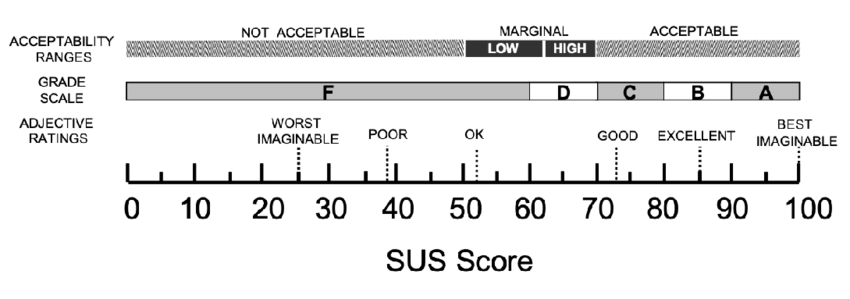
\includegraphics[width=0.8\textwidth]{figures/Grade-rankings-of-SUS-scores-from-An-Empirical-Evaluation-of-the-System-Usability.png}
        \caption{Bare midlertidig bilde.}
        \label{fig:sus_scores}
\end{figure}


With a mean SUS score of \textbf{85.0}, the dashboard is placed in the \emph{excellent} range (95–97\textsuperscript{th} percentile) and well above the industry benchmark of~68. 

Because only three users participated, the results should be seen as an indication rather than a statistically precise measure. However, it is important to highlight that all three participants are the actual target users of the system, and they are the ones who will use the dashboard in practice. 
This indication along with the other results from our user tests leads us to believe that the application design is working as intended and has a high level of usability. 

\begin{table}[H]
\centering
\begin{tabular}{@{}lcc@{}}
\toprule
\textbf{Raw \acrshort{sus} score} & \textbf{Percentile range} & \textbf{Letter grade} \\
\midrule
85 & 95--97\,\% & A (Excellent) \\
\bottomrule
\end{tabular}
\label{tab:sus-benchmark}
\caption{Benchmark interpretation of the mean \acrshort{sus} score}
\end{table}

%vet ikke om det er nødvendig, blir trolig flyttet ned til diskusjon?
\textbf{Qualitative context}

Observation notes and \gls{thinkaloudprotocol} comments highlight a few pain points that the \acrshort{sus} alone cannot pinpoint:

\begin{itemize}
    \item Graph comprehension. Several testers hesitated when interpreting the downtime and performance graphs and asked for clearer legends or time scales.
    \item Navigation shortcuts. Some users expected a more direct route to “Add Website” than the current menu placement.
    \item Alert details. Participants wanted quicker access to incident causes from the alert list.
    \item Icon clarity. The “focus-mode” icon was frequently misunderstood.
\end{itemize}

These qualitative findings align with the few neutral or slightly negative ratings on items that probe complexity and consistency (items 2, 6, 8, 10). For example, confusion about graph labels likely influenced the “too much inconsistency” statement (item 6).

Interpretation and next steps
With a mean \acrshort{sus} of 85, the dashboard comfortably exceeds the accepted usability baseline (68) and sits in the “excellent” bracket. Nevertheless, the test notes point to specific refinements—chiefly clearer data visualisation, more intuitive placement of key actions, and improved iconography—that could push both perceived learnability and satisfaction even higher.

A percentile chart matching raw \acrshort{sus} scores to their ranks is provided...in Appendix ?; Chapter 6 discusses how these usability results informed the final design tweaks before handover.


\section{Refined Requirement Specification}
\label{sec:refined_req_specification}
Table \ref{tab:refined-reqs} lists the consolidated functional (F1–F10)
and non‑functional (NF1–NF6) requirements that guided development and testing.

%Her skal final krav inn, både funksjonelle og ikke funskjonelle




\section{System Overview and Final Implementation}
\label{sec:system_results}

This section describes the final state of the dashboard application at the end of development. It presents the key technical and design outcomes, including system architecture, component behavior, and how stakeholder requirements were addressed in the implementation. Each element is analyzed in relation to established usability and design principles.

\subsection{System Architecture and Sitemap}
\label{subsec:system_sitemap}

The application was structured as a multi-page dashboard system. Figure~\ref{fig:sitemap} presents a sitemap summarizing the key user-accessible components.

\begin{figure}[H]
        \centering
        \includegraphics[width=\textwidth]{figures/Sitemap.png}
        \caption{Application sitemap showing all available pages and views}
        \label{fig:sitemap}
\end{figure}

\subsection{Monitoring Logic and Alert System}
\label{subsec:monitoring_logic_results}

Monitoring functionality was implemented using \texttt{axios} for \gls{http} requests and the \texttt{cron} module for scheduled jobs. Each monitored site was queried at user-defined intervals to collect \gls{http} status and \acrfull{ttfb}. Failure triggered a retry after 60 seconds; consecutive failures logged an incident and triggered an alert.

Users could set performance thresholds. Alerts were sent based on user-defined criteria and email settings. The system supported Norman’s principle of \textit{constraints} and Few’s \textit{critical value exception} by reducing unnecessary notifications and surfacing only relevant anomalies.

\subsection{Incident Tracking System}
\label{subsec:incident_tracking_results}

User feedback from Test 2 resulted in the implementation of Requirement F.11, the Incident System. Incidents are created for consecutive failures and elevate the affected website card within the dashboard. Users can explore incidents in a dedicated list or on the relevant website’s details page.

\subsection{User Authentication}
\label{subsec:user_authentication_results}

Authentication was not initially planned but added in response to user feedback. Implemented using \texttt{jsonwebtoken}, it enables secure login, registration, and personalized dashboards.

\subsection{User Interface Design and Behavior}

\subsubsection{Dashboard Page}
\label{subsubsec:dashboard_results}

The dashboard was designed according to Few’s principles of simplicity and Nielsen's heuristic of aesthetic and minimalist design. It prioritizes actionable data, using dynamic ordering of components, status indicators, and color-coded alerts. Gestalt principles such as proximity, enclosure, and similarity structure the interface visually.

\subsubsection{Website Card Component}
\label{subsubsec:website_card_results}

The card component reflects a website’s live status. It adapts based on monitoring results and is color-coded for instant readability. Consistent styling and iconography reduce cognitive load and support both Norman's and Nielsen’s views on consistency  \theoryref{par:consistency_and_standards}{Nielsen1994}.

\begin{figure}[H]
    \centering
    \includegraphics[width=1\linewidth]{figures//MVP-dashboard/MVP-cards.png}
    \caption{Visual comparison of the Website Card component in online and offline states}
    \label{fig:websitecard-comparison}
\end{figure}

\subsubsection{Website Details Page}
\label{subsubsec:website_details_results}

This page supports deeper analysis of individual websites. It includes performance trends, incident history, and visual alerts. Its design emphasizes visibility, affordance, and feedback. Filters, status indicators, and banner alerts ensure users are aware of key system changes.

\begin{figure}[H]
    \centering
    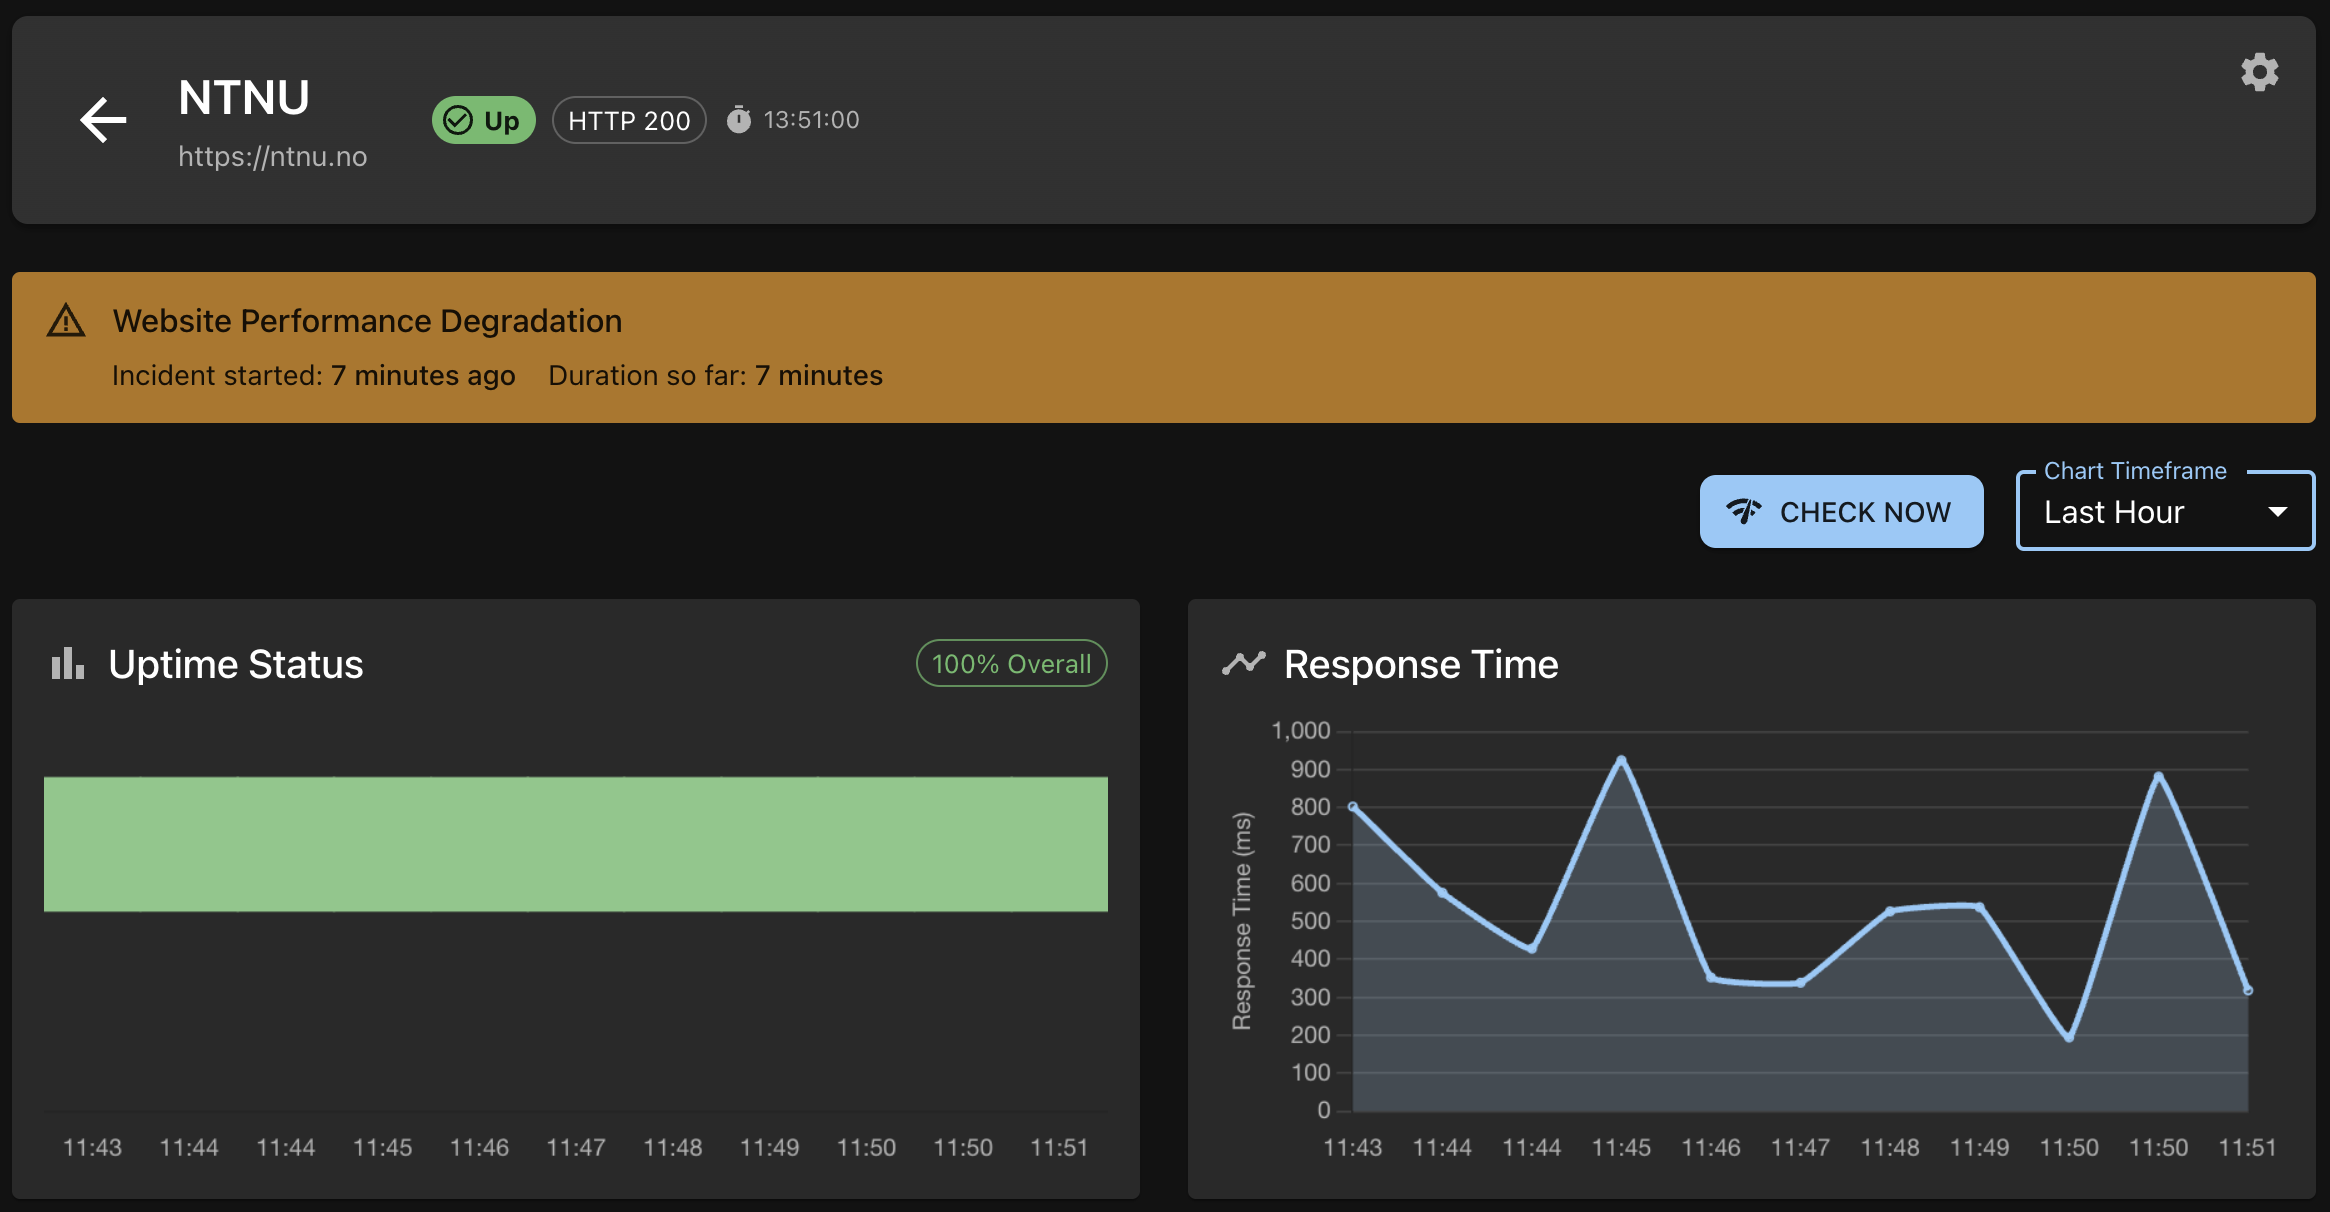
\includegraphics[width=1\linewidth]{figures/websiteDetails.png}
    \caption{Website details with charts and incident highlights}
\end{figure}

\begin{figure}[H]
    \centering
    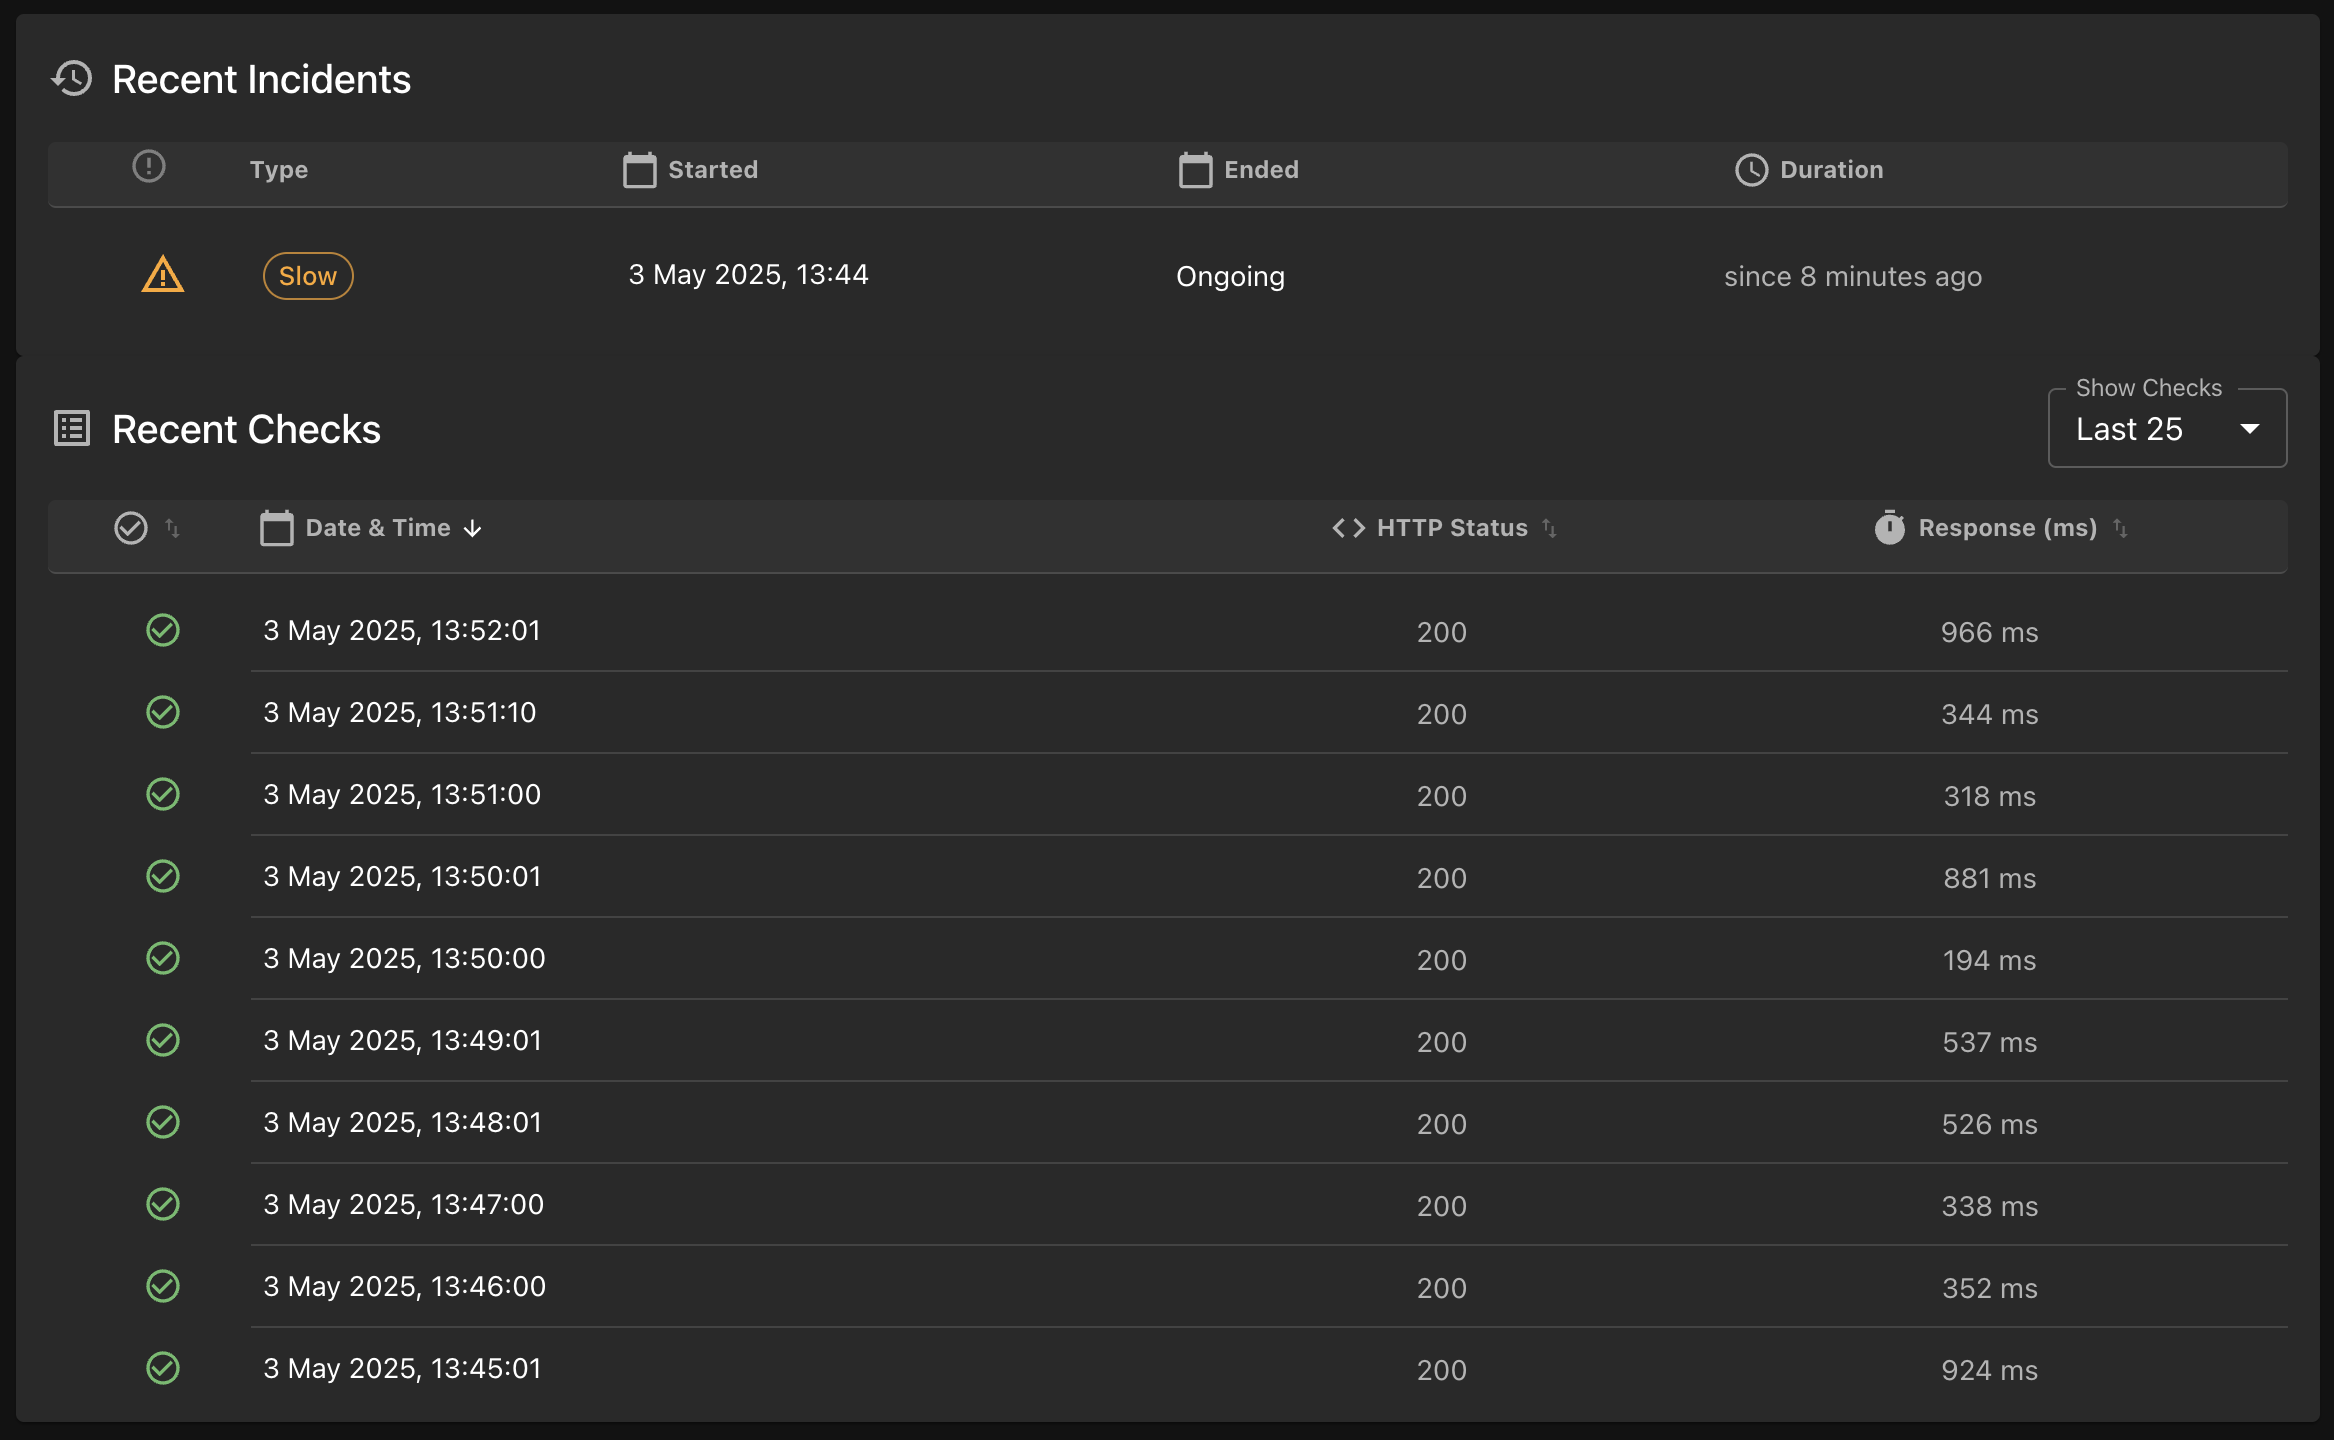
\includegraphics[width=1\linewidth]{figures/websiteDetails_bottom.png}
    \caption{Lower section of website details page with incident timeline}
\end{figure}

\subsection{Requirement Fulfillment Summary}
\label{subsec:req_fulfillment_results}

Most core requirements were met. Below is a fulfillment breakdown:

\begin{itemize}
    \item \textbf{Fully met:} F.1–F.4, F.6–F.8; NF.1–NF.3.
    \item \textbf{Partially met:}
    \begin{itemize}
        \item F.5 - Authentication added; role-based access not implemented.
        \item F.9 - Interval configuration exists; server-side limits not enforced.
        \item NF.4 - Documentation exists, but lacks depth.
    \end{itemize}
    \item \textbf{Not implemented:} NF.5 - Responsive layout exists but lacks full mobile optimization.
    \item \textbf{Added post-testing:} F.11 - Incident system.
\end{itemize}

\subsection{Summary of System Results}
The monitoring dashboard application met nearly all planned requirements and additional user-suggested features. Its final form balances usability and functionality, grounded in established UI design theory. Together, the monitoring logic, incident management, and dynamic UI produce a system capable of real-time, intuitive operational awareness.

